% LZW Compression Process
\begin{algorithm}[H]
	\caption{LZW Compression Process} 
	\begin{algorithmic}[1]
\State Initialize an empty dictionary.
\State Populate the emptied dictionary with all possible one-length characters from the extended ASCII set (values 0 to 255).
\State Initialize an empty string $\mathbf{P}$.

\While{not at the end of the character stream}
    \State $\mathbf{C = \text{next character}}$.
    \If{$\mathbf{P + C}$ exists in the dictionary}
        \State $\mathbf{P = P + C}$ (Extend by adding C to the string P).
    \Else
        \State Output the code for $\mathbf{P}$.
        \State Append the string $\mathbf{P + C}$ to the dictionary.
        \State $\mathbf{P = C}$ (Replace the string P with the current character).
    \EndIf
\EndWhile
	\end{algorithmic} 
\end{algorithm}

\vspace{10pt}

The compression phase of the LZW algorithm involves scanning through the input data, identifying repeating sequences, and replacing them with shorter codes that refer to these sequences. Initially, the dictionary contains all possible individual symbols that appear in the input data. As the algorithm processes the input, it builds the dictionary dynamically by adding longer sequences of characters encountered during the scan.

\vspace{10pt}

The process starts by taking an input string and checking if it already exists in the dictionary. If the sequence is found, it is replaced with the corresponding code. If the sequence is not found, it is added to the dictionary with a new code, and the algorithm continues with the next symbol. This approach works efficiently when dealing with data that contains a lot of repetitive sequences, as a single code can replace each repeating pattern.

\vspace{10pt}

\textcolor{magenta}{\textbf{Example:}} LZW compression process for the string "\textcolor{Tue-red}{\textbf{ABCBCCAB}}".

\vspace{10pt}

\textbf{Initialize:} Dictionary with all possible single-length characters from the extended ASCII table. Each character serves as the key, and the corresponding value is initialized to 0, for instance: dictionary["0"] = 176, dictionary["A"] = 193.

% \begin{figure}[ht]
%   \centering
%   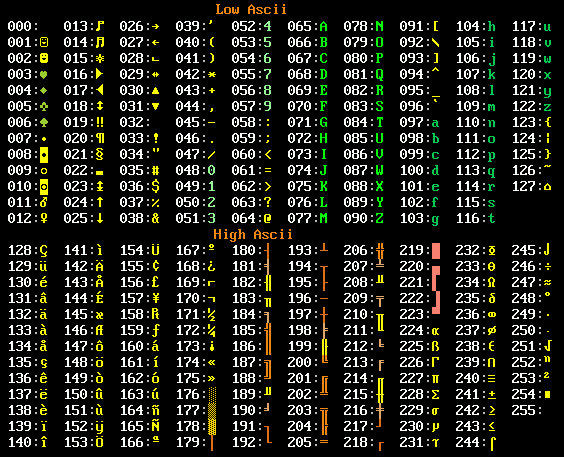
\includegraphics[height=0.5\textwidth]{Figures/ascii.png}
%   % \caption{extended ASCII set}
% \end{figure}

\begin{table}[ht]
    \caption{Trace of the LZW Algorithm step by step: Compression process}
    \centering
\adjustbox{max width=\textwidth}{
\begin{tabular}{|c|c|c|c|c|l|}
\hline
\multirow{2}{*}{\textbf{Step}} & \multicolumn{2}{|c|}{\textbf{Encoder Output}} & \multicolumn{2}{c|}{\textbf{Dictionary}} & \multirow{2}{*}{\textbf{Explaination}} \\ \cline{2-5}
 & \textbf{Output} & \textbf{Represents} & \textbf{Key} & \textbf{Value} & \\ \hline
1 &  &  &  &  & P = "", C = "A", assign P+C = "A" to P \\ \hline
2 & 193 & "A" & "AB" & 256 & P = "A", C = "B",  assign C = "B" to P\\ \hline
3 & 194 & "B" & "BC" & 257 & P = "B", C = "C", assign C = "C" to P \\ \hline
4 & 195 & "C" & "CB" & 258 & P = "C", C = "B", assign C = "B" to P \\ \hline
5 &  &  &  &  & P = "B", C = "C", assign P+C = "BC" to P \\ \hline
6 &  257& "BC" & "BCC" & 259 & P = "BC", C = "C", assign C = "C" to P \\ \hline
7 & 195 & "C" & "CA" & 260 & P = "C", C = "A", assign C = "A" to P \\ \hline
8 &  &  &  &  & P = "A", C = "B", assign P+C = "AB" to P \\ \hline
9 & 256 & "AB" &  &  & P = "AB", C = ""\\ \hline
&   &   &  & & end of stream \\ \hline
\end{tabular}
}

    \label{tab:lzw_trace_compress}
\end{table}

\textbf{Encoder:} The compressor output is the binary form of each column encoder output for characters representation, such as here: \textbf{\textcolor{cyan}{193 194 195 257 195 256}}.




